\documentclass[eng,oneside]{mgr}

\usepackage{polski}

\usepackage[utf8]{inputenc}
\usepackage[T1]{fontenc}

\usepackage{graphicx}
\usepackage{caption}
\usepackage{subcaption}

\usepackage{wrapfig}
\usepackage{psfrag}

\usepackage{amsmath}
\usepackage{amsfonts}

\usepackage{listings}
\usepackage{url}

\title{Mikroprocesorowy Sterownik Rotora Antenowego}
\engtitle{Microprocessor controller for antenna rotor}
\author{Paweł Marcin Szwagierek}
\supervisor{dr inż. Jerzy Greblicki, I-6}
\date{2013}

\field{Informatyka (INF)}
\specialisation{Inżynieria internetowa (INT)}

\makeatletter
\def\@makechapterhead#1{%
  \vspace*{50\p@}%
  {\parindent \z@ \raggedright \normalfont
    \ifnum \c@secnumdepth >\m@ne
      \if@mainmatter
        \Huge\bfseries \thechapter.\space%
      \fi
    \fi
    \interlinepenalty\@M
    \Huge \bfseries #1\par\nobreak
    \vskip 40\p@
  }}
\makeatother 

\begin{document}
	\bibliographystyle{plabbrv} 
	\maketitle

	\tableofcontents

	\chapter{Wstęp}
	Celem projektu jest zbudowanie sterownika rotora antenowego dla zastosowań krótkofalarskich. Główną jego ideą jest automatyczne śledzenie trajektorii satelitów podczas amatorskich łączności krótkofalarskich. 

	W obecnych czasach krótkofalarstwo jest domeną pasjonatów i hobbystów. Ludzie, którzy chcą bawić się sprzętem radiowym i komunikować się z różnymi częściami świata bądź swoimi bliskimi przyjaciółmi, gotowi są zainwestować w tę pasję duże ilości swojego czasu i pieniędzy. Te pasję z kolei łączą z różnymi innymi aktywnościami, na przykład zdobywanie szczytów górskich czy wyprawy w niezdobyte lub niezamieszkałe tereny. Czasami podczas takich wypraw konwencjonalne łączności krótkofalarskie są niemożliwe. Wtedy radioamator próbuje skorzystać w próbach nawiązania łączności na dalekie odległości ze zjawisk naturalnych (jak zorze polarne) lub z infrastruktury stworzonej przez samych hobbystów (amatorskie satelity krótkofalarskie krążące na niskich orbitach nad Ziemią). Jednak aby wykorzystać takie możliwości, trzeba mieć do tego odpowiedni sprzęt. Profesjonalne akcesoria do łączności satelitarnych są drogie i mało praktyczne w czasie dalekich wypraw na górskie szczyty lub nawet krótkich wycieczek poza miasto. Istnieją także tanie rozwiązania które są jednak one trudne w obsłudze, zwłaszcza w sytuacji gdy operator takiej terenowej stacji musi skupić się na prawidłowym wykonaniu łączności.

	Poniższa praca skupia się na rozwiązaniu tego problemu. W rozdziale~\ref{sec:teoretical_description} przytoczone zostały ważne pojęcia związane z pracą i wielokrotnie w niej używane. W części~\ref{sec:problem_description} sformułowany został problem, który będzie rozwiązywany i zostały przedstawione jego główne założenia. Rozdział~\ref{sec:existing_possibilities} będzie swego rodzaju przedstawieniem różnych możliwości, które mogłyby być wykorzystane do rozwiązania postawionego problemu. Treść rozdziału~\ref{sec:project_realization} będzie przedstawieniem kolejnych etapów prac nad projektem. Opisane zostały poszczególne zagadnienia, urządzenia oraz sposób ich wykorzystania w projekcie. Przedstawiona została także konfiguracja każdego z modułów zastosowanego mikrokontrolera. W rozdziale~\ref{sec:how_to_use_device} opisana została poprawna obsługa i użycie urządzenia, a także konfiguracja niezbędnego oprogramowania komputerowego. Rozdział~\ref{sec:summit} będzie podsumowaniem pracy, opisem dodatkowych możliwości rozwoju projektu oraz jego słabych punktów.

	\chapter{Problematyka amatorskich systemów radiowych}
	\label{sec:teoretical_description}
	TODO
		
		\section{Radioamator}
		Osoba zajmująca się radiotechniką niezawodowo. Istnieją radioamatorzy bierni, poprzestający na studiowaniu samego tematu krótkofalarstwa, rzadko wkraczający w~dziedzinę praktyki radioamatorskiej. Amatorzy czynni na podstawie zezwolenia odpowiednich władz budują i~uruchamiają własne, indywidualnie lub zbiorowo, krótkofalowe i~ultrakrótkofalowe stacje nadawcze małej mocy.

		Tacy radioamatorzy, wymieniając ze swymi kolegami w~kraju i~za granicą doświadczenia i~spostrzeżenia dotyczące techniki radioamatorskiej, rozprzestrzeniania się fal elektromagnetycznych w~poszczególnych zakresach itp., przyczyniają się niejednokrotnie do rozwoju wiedzy i~techniki. 

		\section{Krótkofalarstwo}
		Terminem krótkofalarstwo określa się hobby polegające na nawiązywaniu łączności z~innymi stacjami radioamatorskimi za pomocą nadajników radiowych. W~przypadku nowoczesnych sposobów komunikacji (np. poczta elektroniczna, komunikatory internetowe, telefonia komórkowa), nieważny jest sposób przesłania informacji z~punktu A do punku B, a sama informacja. W wypadku krótkofalarstwa większy nacisk kładzie się na sposób przesłania informacji (sprzęt radiowy, rodzaj emisji, pasmo, anteny itd). Podczas samych łączności krótkofalarskich istotnymi informacjami wymienianymi przez użytkowników stacji są ich osobiste znaki wywoławcze oraz raporty o~słyszalności i~sile odebranego sygnału. Samo krótkofalarstwo jest dziedziną zainteresowań o~bogatym wachlarzu możliwości. 

			\subsection{Edukacja}
			Jednym z~korzyści jakie niesie ze sobą ten temat, to ogromna ilość wiedzy z~różnych lecz poniekąd pokrewnych sobie dziedzin. Taka wiedza może zostać przekazana uczniom szkół w~czasie zajęć obejmujących zagadnienia ściśle powiązane z~krótkofalarstwem. Bogatą wiedzę można także pozyskać uczestnicząc w~spotkaniach klubów krótkofalarskich lub uczestnicząc w~zajęciach prowadzonych przez takie kluby. Przekazywane tam informacje są najbardziej usystematyzowane. Rozwiązanie takie daje także możliwości skorzystania z~klubowych radiostacji. Ostatnim ze sposobów podjęcia takiej wiedzy jest nauka samodzielna korzystając z~rozmaitej literatury tematycznej, publikacji lub artykułów sporządzonych samodzielnie przez radioamatorów z~całego świata. 

			Przede wszystkim radioamator uczy się przy okazji pasji dużo z~dziedziny telekomunikacji. Poznaje rodzaje anten, które wykorzystuje się w~pracy z~różnymi pasmami a także ich budowę. Uczy się także typów modulacji oraz rodzajów emisji. W~przypadku elektroniki krótkofalarstwo daje szansę poznania zasad działania różnych urządzeń elektronicznych oraz zagadnienia przetwarzania sygnałów. Budowanie automatycznych przełączników lub sterowników rotorów antenowych wiąże się z~poznaniem zagadnień z~dziedziny automatyki. Krótkofalarstwo wprowadza także wiele wiedzy z~zakresu informatyki, gdzie radioamator może wykorzystać do transmisji informacji różne rodzaje emisji cyfrowych lub stworzyć swój własny system SDR\footnote{SDR (ang. Software Defined Radio, radio definiowane programowo) – system komunikacji radiowej, w~którym działanie podstawowych elementów elektronicznych (takich jak mieszacze, filtry, modulatory i~demodulatory) jest realizowane za pomocą programu komputerowego.} i~korzystać ze swojego oddalonego o~znaczną odległość radia za pośrednictwem Internetu lub dać możliwość korzystania ze swoich anten i~prowadzenia nasłuchu innym radioamatorom. Na pograniczu leżą także takie dziedziny nauki jak kryptografia, w~przypadku gdy użytkownicy dwóch stacji chcą się porozumiewać zachowując poufność przesyłanych informacji. Istotną umiejętnością jest także znajomość języków obcych. Bez tego prawie niemożliwym jest prowadzenie łączności z~radioamatorami posługującymi się innymi językami.

			Jest to jedna z~nielicznych pasji, która pozwala na wykorzystanie własnoręcznie stworzonego sprzętu. Społeczność krótkofalowców popiera i~wręcz dopinguje budowanie i~wykorzystanie własnych urządzeń radiowych, anten a także pozostałego oprzyrządowania niezbędnego w~pracy lub ułatwiającego pracę radioamatora - jak na przykład przełączniki antenowe, wzmacniacze, klucze telegraficzne itp). Dodatkowym atutem jest brak konieczności posiadania jakichkolwiek homologacji lub zezwoleń na korzystanie z~własnych urządzeń. Najwięcej osób używa jednak urządzeń fabrycznych. Jest to droższe rozwiązanie, ale dużo łatwiejsze aby od razu zacząć 

			\subsection{Amatorska Służba Radiowa}
			\begin{wrapfigure}{r}{0.4\textwidth}
				\vspace{-20pt}
				\begin{center}
					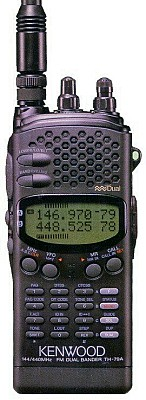
\includegraphics[scale=0.5]{ukf_handheld}
				\end{center}
				\vspace{-20pt}
				\caption{Prosty nadajnik ręczny do pracy w~paśmie UKF}
				\vspace{-40pt}
				\label{fig:ukf_handheld}
			\end{wrapfigure}
			Radioamatorzy posiadający urządzenia nadawczo-odbiorcze są w~stanie skomunikować się ze znaczną grupą osób w~swoim otoczeniu lub dowolnym zakątkiem kraju czy świata. To daje możliwość pomocy innym ludziom w~wymianie informacji w~sytuacjach nieprzewidzianych, nagłych wypadkach, katastrofach lub klęskach żywiołowych. Krótkofalowcy są często jedynymi, którym udaje się nawiązać łączność pomiędzy odciętymi komunikacyjnie regionami. Wielu radioamatorów angażuje się także w~szkolenie innych ludzi w~zakresie krótkofalarstwa lub dziedzin ściśle z~nim powiązanych. To pozwala łatwiej zacząć przygodę z~krótkofalarstwem.

			\subsection{Hobby}
			Najwięcej ludzi skłania się do krótkofalarstwa z~powodu hobby. Posiada wiele dyscyplin jak zawody, wyprawy, prowadzenie łączności dalekiego zasięgu, eksperymentowanie z~różnymi typami emisji lub po prostu pozostawanie w~kontakcie z~przyjaciółmi korzystając z~innego środka komunikacji od popularnych w~dzisiejszych czasach telefonii komórkowej czy Internetu.

				\subsubsection{Łączności lokalne}
				Do prowadzenia łączności ze znajomymi mieszkającymi w~naszym otoczeniu wystarczy tani nadajnik przenośny pokazany na rysunku~\ref{fig:ukf_handheld} lub samochodowy pracujący na pasmach UKF. Stosunkowo mała moc urządzeń pozwala na objęcie swoim zasięgiem czasami nawet całego miasta. W~przypadku gdy taki zasięg staje się niewystarczający, w~orężu radioamatorów pozostają tzw. przemienniki - urządzenia montowane na znacznych wysokościach (wysokich obiektach miejskich, wzniesieniach terenu), które odbierają sygnał i~nadają go powtórnie z~większą mocą. Skutkuje to wielokrotnym zwiększeniem zasięgu prowadzonych łączności nawet do kilkuset kilometrów. Przemienniki amatorskie nie nadają cały czas, aby nie zużywały energii gdy nikt z~nich nie korzysta. W~celu skorzystania z~takiego przemiennika należy go wcześniej ,,otworzyć'' sygnałem akustycznym o~określonej częstotliwości, jednym z~tonów DTMF lub sygnałów CTCSS

				\subsubsection{Łączności dalekiego zasięgu (DX)}
				Radioamatorzy, którzy korzystają z~bardziej zaawansowanych urządzeń i~anten mogą pracować z~innymi rodzajami emisji oraz na innych pasmach (fale krótkie (KF), fale średnie). Pozwala to na realizację łączności na dużo większe odległości - opierając się na samej mocy i~charakterystyce emitowanego sygnału, wykorzystując zjawiska pogodowe, zjawisko odbicia fal lub korzystając z~amatorskich satelitów komunikacyjnych działających w~paśmie UKF. Można dzięki temu nawiązywać łączności międzykontynentalne na dystansach rzędu tysięcy kilometrów.
					
					\paragraph{Fale odbite od warstw jonosfery}
					Łączności dalekiego zasięgu na falach krótkich można zrealizować korzystając z~nadajników małej mocy i~nieskomplikowanych drutowych anten wykorzystując zjawisko odbicia fal od jonosfery. Zjawisko to występuje powszechnie i~w~zależności od pory dnia i~aktywności słonecznej umożliwia łączności na odległość od kilkuset to kilkunastu tysięcy kilometrów. Łączności z~najbardziej odległymi stacjami prowadzi się poprzez wielokrotne odbicia, niekiedy pokonujące dłuższą drogę wokół kuli ziemskiej.

					\paragraph{Fale odbite od powierzchni księżyca}
					\begin{wrapfigure}{r}{0.4\textwidth}
						\vspace{-20pt}
						\begin{center}
							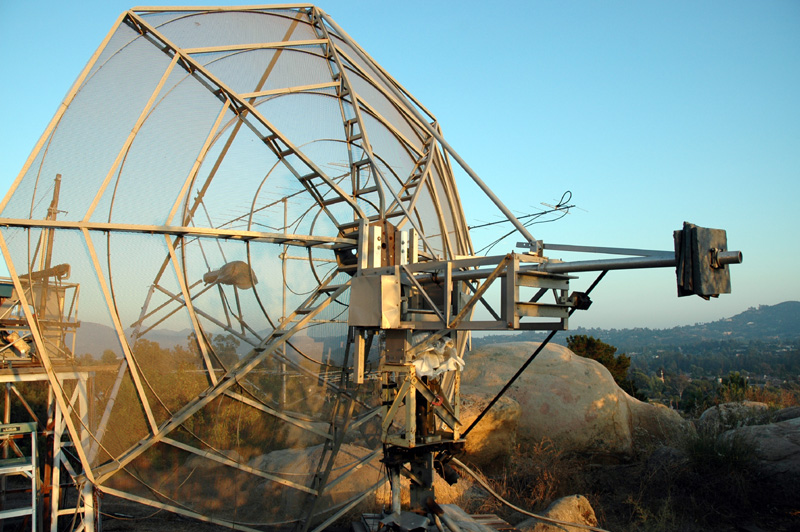
\includegraphics[width=0.4\textwidth]{eme_antenna}
						\end{center}
						\vspace{-20pt}
						\caption{Antena paraboliczna wykorzystywana do łączności EME pracująca w~paśmie fal 430MHz}
						\vspace{-10pt}
						\label{fig:eme_antenna}
					\end{wrapfigure}
					Jednym z~najbardziej niezwykłych rodzajów łączności są te z~wykorzystaniem odbicia fali od powierzchni księżyca (EME). Do tego typu łączności wykorzystuje się zaawansowane systemy antenowe (jak przedstawiona na rysunku~\ref{fig:eme_antenna} oraz nadajniki o~wysokiej mocy. Przy EME wymagana jest duża precyzja oraz doświadczenie w~prowadzeniu takich łączności, przez co jest to dziedzina krótkofalarstwa która odstrasza początkujących radioamatorów. 


					Antena powinna być skierowana dokładnie w~kierunku księżyca, który pozostaje w~ruchu względem powierzchni ziemi. W~związku z~tym aby powszechnie wykorzystywanymi są skomplikowane systemy obracania anten. W~przypadku złego ustawienia anteny najczęstszymi zakłóceniami sygnału są zniekształcenia czoła fali w~wyniku nakładania się fal odbitych. Typowymi dla tego rodzaju łączności są zjawiska odbioru własnego echa po około 2 sekundach od wysłania komunikatu oraz niewyjaśnione dotąd zjawisko echa z~dużym opóźnieniem. Skutkiem tego jest otrzymanie przez nadawcę swojego komunikatu ale po czasie dochodzącym nawet do kilku minut.

					Łączności wykonywane tą techniką ze względu na małą skuteczność, małą pewność transmisji oraz trudności związane z~jej wykonaniem realizują tylko radioamatorzy.

					\paragraph{Łączności satelitarne}
					\begin{wrapfigure}{r}{0.4\textwidth}
						\vspace{-20pt}
						\begin{center}
							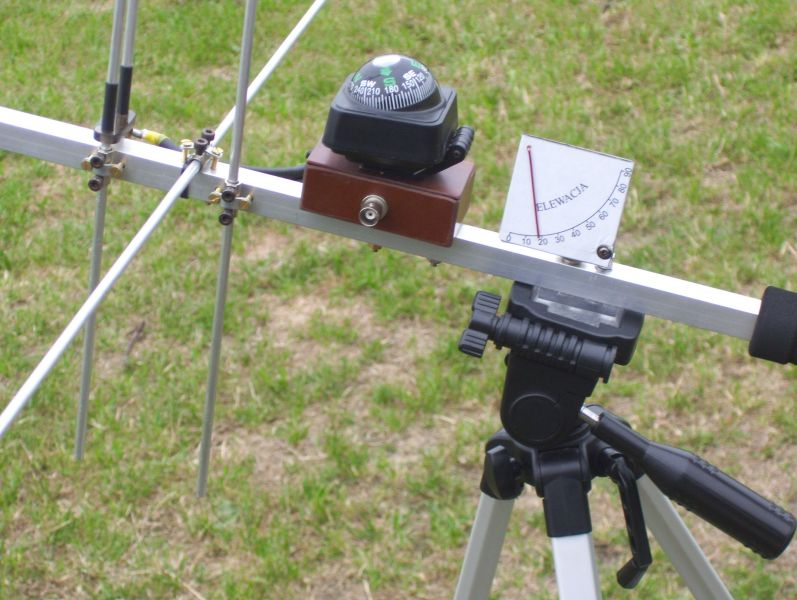
\includegraphics[width=0.4\textwidth]{example_sat_construction}
						\end{center}
						\vspace{-20pt}
						\caption{Konstrukcja radioamatora SQ5RJK do ręcznego ustawiania i~korygowania pozycji anteny podczas łączności satelitarnych}
						\vspace{-10pt}
						\label{fig:example_sat_construction}
					\end{wrapfigure}
					Krótkofalowcy korzystają także ze swoich satelitów. Takich satelitów niskoorbitalnych\footnote{Satelita niskoorbitalny - satelita krążący wokół Ziemi po orbicie kołowej na wysokości 10 tys. km - 500 tys. km} jest kilkadziesiąt i~co jakiś czas wysyłane są kolejne. Fale pasma UKF pozwalają na przeprowadzenie łączności z~astronautami z~międzynarodowej stacji kosmicznej ISS a także na łączności pomiędzy radioamatorami. Korzystanie z~satelitów wymaga znajomości ich pozycji na niebie, parametrów pracy oraz ciągłego korygowania ustawienia anteny. Także sama komunikacja wygląda nieco inaczej niż w~przypadku normalnej łączności. W~przypadku satelity wiadomości nadawane są na częstotliwości zwanej ,,uplink'' i~odbierane na częstotliwości oznaczonej jako ,,downlink''. Jest to uwarunkowane zasadą pracy satelity. Odbiera ona sygnały z~jednej częstotliwości i~retransmituje te same sygnały ze zwiększoną mocą na innej częstotliwości - podobnie jak to dzieje się w~przypadku przemienników amatorskich.
					W~związku z~tym, że pozycja anteny musi być na bieżąco korygowana, stosuje się skomplikowane systemy obracania anten lub rolę tę przejmuje sam radioamator i~pozycję anteny koryguje ręcznie korzystając z~takich konstrukcji jak pokazana na rysunku~\ref{fig:example_sat_construction}


					\paragraph{Inne typy łączności}
					Sporadycznie radioamatorzy korzystają do zrealizowania łączności z~takich zjawisk jak odbicia fal radiowych od zorzy polarnej, meteorytów a nawet chmur burzowych.

				\subsubsection{QSL}
				Podstawowym potwierdzeniem każdej wykonanej łączności jest wymiana znaków wywoławczych operatorów stacji oraz wymiana raportów słyszalności i~siły sygnału. To wystarczy, żeby uznać łączność za zrealizowaną. Oficjalnym i~bardzo eleganckim potwierdzeniem łączności są karty QSL\footnote{QSL - Jeden z~symboli Kodu Q używanego w~telegrafii i~krótkofalarstwie. Domyślnym jego znaczeniem jest potwierdzenie łączności.}. Są wizytówkami radioamatorów oraz kartami z~dokładnym opisem zrealizowanej łączności. Dla pewnej grupy krótkofalowców stanowią one swego rodzaju trofea ze swojej służby radiowej. Wielu z~nich skupia się na ustanawianiu łączności z~jak największą ilością stacji z~odrębnych krajów. Jest to ciekawe wyzwanie z~tego powodu, że wraz ze ,,zdobywaniem'' kolejnych krajów, stopień trudności znacząco rośnie, ponieważ istnieją kraje, w~których liczba radioamatorów jest bardzo mała, region kuli ziemskiej uznany w~społeczeństwie krótkofalarskim jako kraj jest niezamieszkały lub ze względów politycznych działalność krótkofalarska nie może funkcjonować.
				\subsubsection{Zawody}
				Jedną z~dziedzin rywalizacji pomiędzy radioamatorami są zawody przeprowadzane w~ściśle określonym czasie. Polegają na nawiązaniu jak największej liczby łączności z~innymi operatorami stacji i~tym samym zdobywaniu punktów przydzielanych według zasad określonych w~regulaminie. Zaliczane są tylko bezbłędne łączności potwierdzone wymienionymi znakami wywoławczymi oraz raportami o~słyszalności. Te dane po zakończeniu zawodów poddawane są weryfikacji przez organizatora przy pomocy programów komputerowych. Zwykle nagrodami są dyplomy dla osoby lub drużyny wygrywającej zawody.

				\subsubsection{Wyprawy}
				W~społeczności krótkofalarskiej popularnymi są także wyprawy zwane inaczej DXpedycjami. Radioamatorzy w~pojedynkę lub w~zorganizowanej grupie wraz z~członkami klubu zdobywają górę lub niezamieszkały teren aby tam utworzyć tymczasową stację i~przeprowadzić łączności z~innymi stacjami.

		\section{Modulacja Szerokości Impulsu (PWM)}
		Sposób regulowania sygnału prądowego lub napięciowego polegający na generowaniu sygnału o stałej amplitudzie i stałym okresie sygnału, lecz zmiennym współczynniku jego wypełnienia (zmiennej szerokości impulsów sygnału). Na rysunku~\ref{fig:pwm} pokazany został przykład regulacji napięcia za pomocą zmiennego współczynnika wypełnienia sygnału. 

		\begin{figure}[!htb]
			\begin{center}
				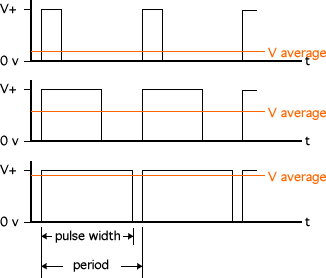
\includegraphics[scale=0.8]{pwm}
			\end{center}
			\caption{Regulacja napięcia sygnałem PWM}
			\label{fig:pwm}
		\end{figure}
		
		Sygnały PWM najczęściej wykorzystywane są do:
		\begin{itemize}
		 	\item zmiany jasności świecenia diod LED,
		 	\item zmniejszania prędkości silników prądu stałego,
		 	\item zmiany jasności podświetlenia wyświetlaczy LCD,
		 	\item sterowania serwomechanizmami modelarskimi,
		 	\item generowania sygnałów analogowych (w tym dźwięków).
		 \end{itemize} 

		\section{Modulacje}
		Modulacja jest to samorzutna lub celowa zmiana parametrów sygnału. W~kontekście krótkofalarstwa modulacja pozwala na nakładanie sygnału wejściowego (niosącego istotne dane jak na przykład głos lub dane cyfrowe do wysłania drogą radiową). Podczas prowadzenia łączności za pomocą fonii, sygnałem wejściowym (modulującym) jest sygnał zawarty w~przedziale 300Hz - 3kHz, czyli zakres częstotliwości fal sygnału mowy. Ten sygnał moduluje falę nośną o~określonej częstotliwości. W~ten sposób powstaje zmodulowany sygnał, gotowy do wypromieniowania w~przestrzeń za pomocą odpowiedniej anteny.
		Poniżej przedstawione zostały modulacje wykorzystywane w~krótkofalarstwie.
			
			\subsection{AM - Modulacja amplitudy}
			\begin{figure}[!htb]
				\begin{center}
					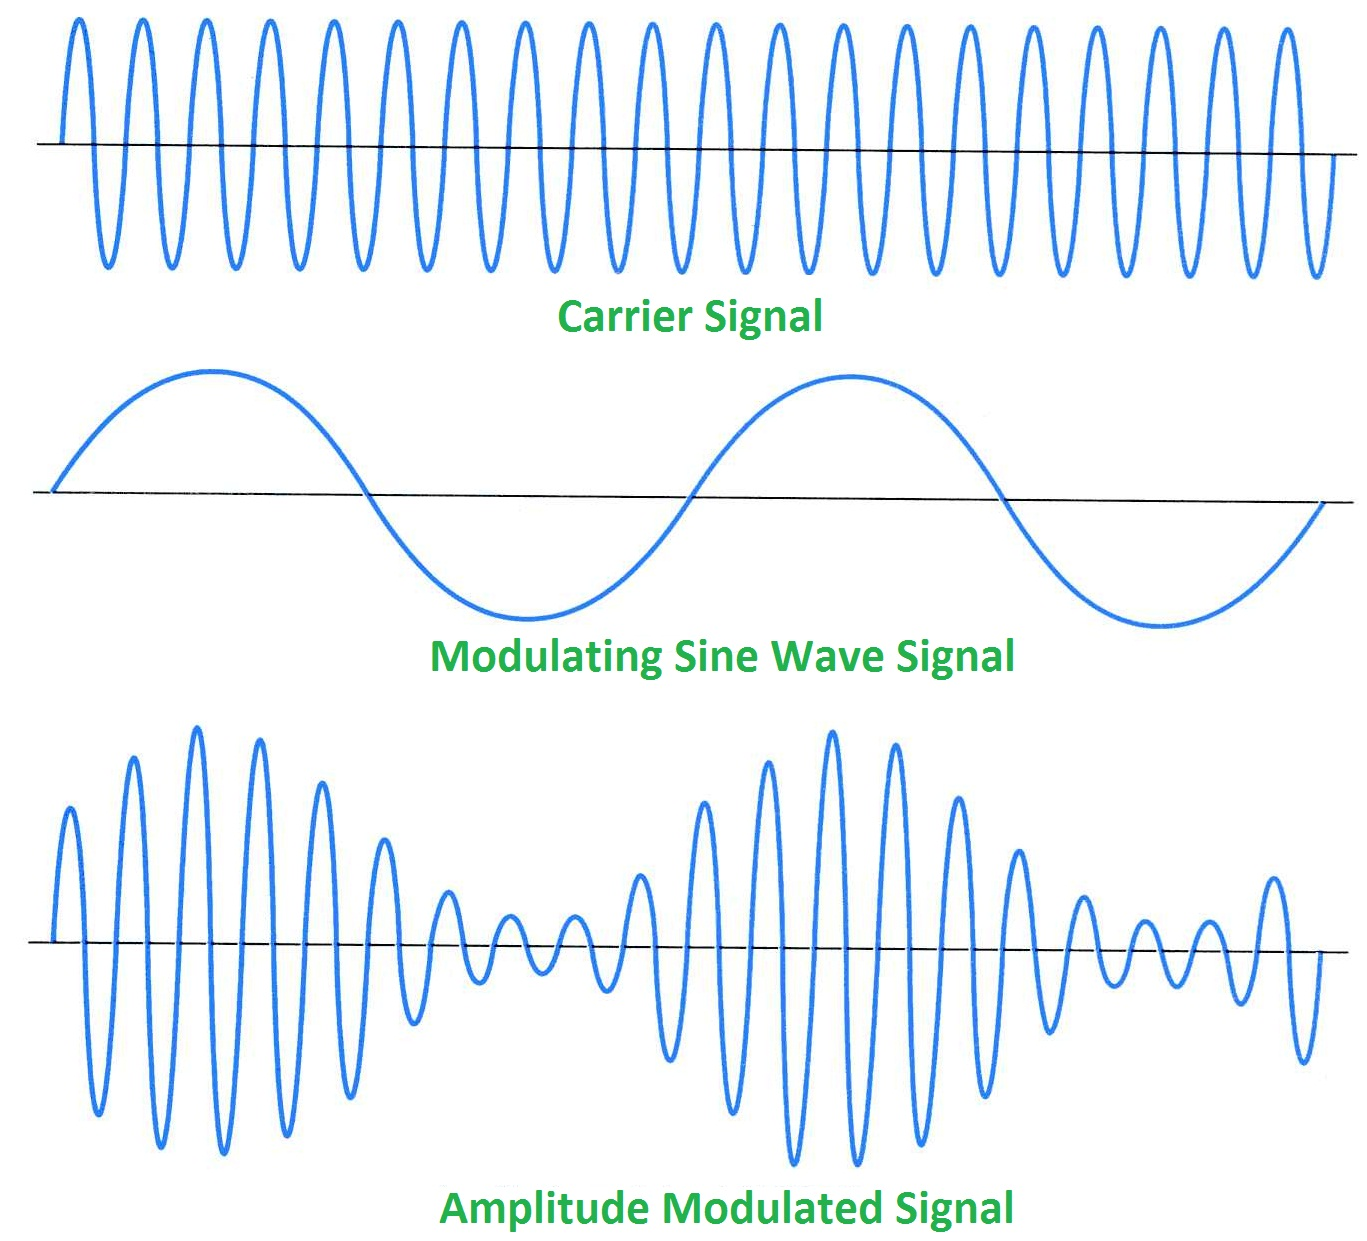
\includegraphics[scale=0.8]{modulacja_am}
				\end{center}
				\caption{Modulacja amplitudy fali nośnej sygnałem sinusoidalnym}
				\label{fig:am_modulation}
			\end{figure}
			Modulacja amplitudy polega na takim przekształceniu fali nośnej sygnałem modulującym, aby wynikiem był sygnał o~częstotliwości fali nośnej i~amplitudzie sygnału modulującego. Szerokość takiego sygnału zmodulowanego jest równa podwojonej częstotliwości modulującej - czyli w~przypadku fonii 6kHz. Całkowita moc wyjściowego sygnału składa się w~50\% mocy nadajnika fali nośnej oraz mocy dwóch wstęg bocznych - po 25\% mocy nadajnika każda. Graficzne przedstawienie takiej modulacji pokazane jest na rysunku~\ref{fig:am_modulation}, gdzie fala nośna została zmodulowana sygnałem sinusoidalnym. 

			\subsection{SSB - Modulacja amplitudy z~wytłumioną wstęgą nośną}
			Modulacja SSB jest szczególnym przypadkiem modulacji amplitudy. W~przypadku czystej modulacji AM moc nadajnika wykorzystywana jest w~50\% przez falę nośną oraz po 25\% przez każdą ze wstęg bocznych sygnału. W~modulacji SSB wytłumiona jest fala nośna oraz jedna ze wstęg bocznych. Skutkiem tego cała moc nadajnika przeznaczona jest wyłącznie na jedną wstęgę boczną modulacji amplitudy sygnału. Dodatkowymi zaletami takiej modulacji jest węższe pasmo częstotliwości emitowanej przez nadajnik, zawężenie o~50\% pasma w~odbiorniku a także mniejszą zawartość sygnałów niepożądanych i~harmonicznych wypromieniowanych przez nadajnik. Niestety te zalety wymagają nadajników o~znacznie bardziej skomplikowanych układach. 

			\subsection{FM - Modulacja częstotliwości}
			Przy modulacji częstotliwości amplituda sygnału pozostaje stała i~jest równa amplitudzie fali nośnej. Pod względem amplitudy sygnału wejściowego zmienia się natomiast częstotliwość generowanego sygnału. Związanym z~modulacją częstotliwości jest pojęcie dewiacji sygnału (inaczej odchylenia częstotliwości). Dewiacją nazywamy różnicę pomiędzy najwyższą i~najniższą częstotliwością fali nośnej w~trakcie modulacji. Jedną z~zalet modulacji częstotliwości sygnału jest większa niż dla modulacji AM odporność na zakłócenia zewnętrzne, zwykle zmieniające chwilową amplitudę sygnału. Kolejną zaletą jest to, że moc sygnału FM nie zmienia się w~procesie modulacji i~jest równa mocy niemodulowanej fali nośnej. Dzięki temu cała moc nadajnika wykorzystywana jest do przekazywania informacji. Przykład modulacji częstotliwości pokazuje rysunek~\ref{fig:fm_modulation}. 
			\begin{figure}[!htb]
				\begin{center}
					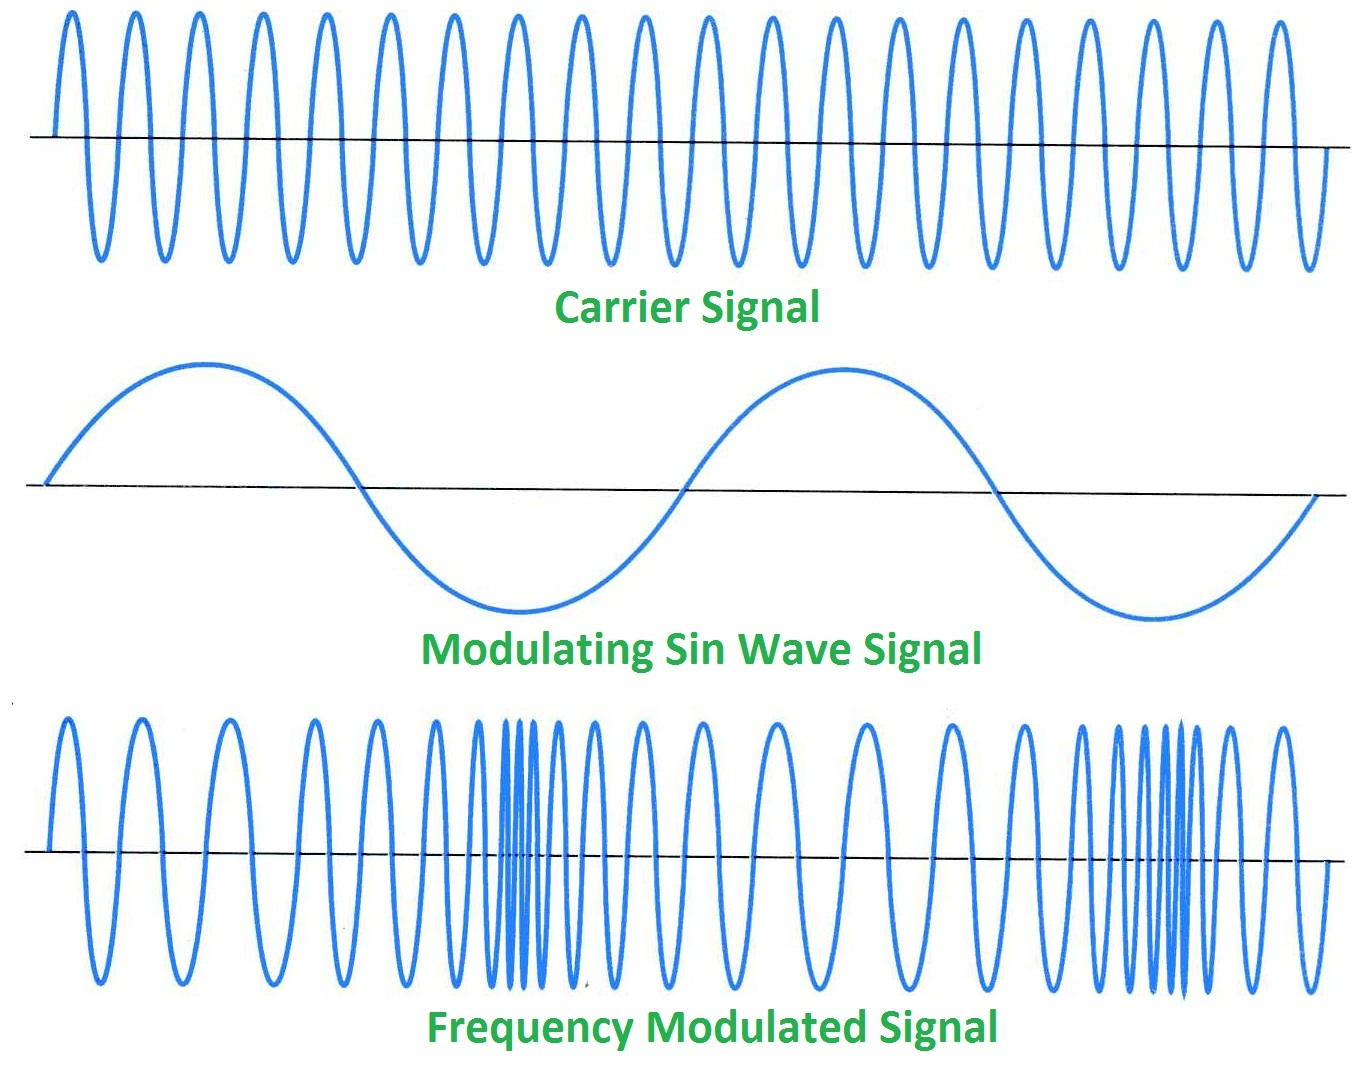
\includegraphics[scale=0.8]{modulacja_fm}
				\end{center}
				\caption{Modulacja częstotliwości fali nośnej sygnałem sinusoidalnym}
				\label{fig:fm_modulation}
			\end{figure}
		
	\chapter{Opis problemu}
	\label{sec:problem_description}
	\begin{wrapfigure}{r}{0.6\textwidth}
		\vspace{-20pt}
		\begin{center}
			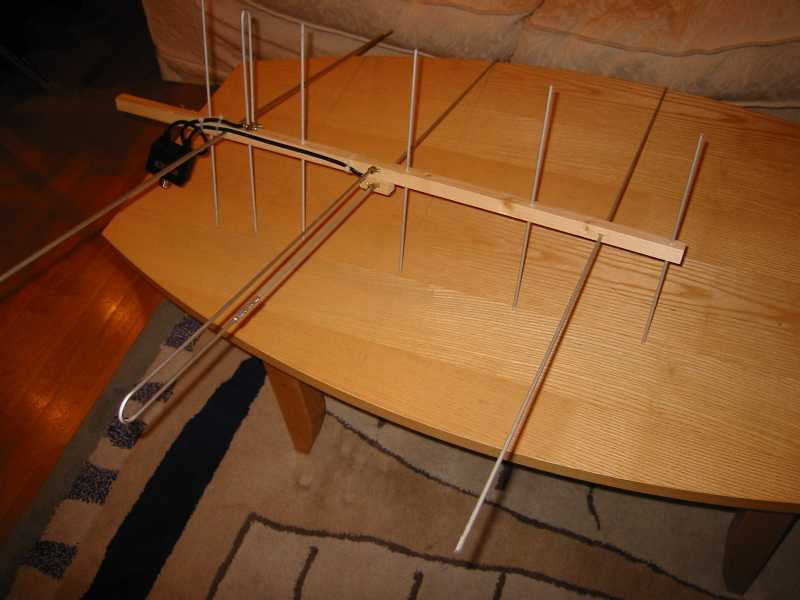
\includegraphics[width=0.55\textwidth]{arrow1}
		\end{center}
		\vspace{-20pt}
		\caption{Ręczna antena Arrow do łączności satelitarnych, przygotowana do transmisji na paśmie 2m i~70cm}
		\vspace{-20pt}
		\label{fig:example_handheld_arrow_antenna}
	\end{wrapfigure}
	Ciekawym połączeniem hobby krótkofalowców są wyjazdy połączone z~prowadzeniem łączności satelitarnych. Łączności takie realizowane są często wykorzystując nadajniki małej mocy. Wymagane do tego są ręczne lub przenośne dwupasmowe nadajniki VHF/UHF (pracujące na falach ultrakrótkich\footnote{UKF (Ultra Krótkie Fale) - zakres fal radiowych o~częstotliwości 30MHz - 300MHz, co odpowiada długości fali 1m - 10m. W~języku angielskim oznaczane jako VHF (Very High Frequency).} i~decymetrowych\footnote{Fale decymetrowe - zakres fal radiowych o~częstotliwości 300MHz - 3GHz, co odpowiada długości fali 10cm - 100cm. W~języku angielskim oznaczane jako UHF (Ultra High Frequency).}). Na takie wyjazdy radioamatorzy przygotowują ręcznie skonstruowane lub zakupione lekkie anteny Arrow (rys.~\ref{fig:example_handheld_arrow_antenna}). Profesjonalne anteny do komunikacji satelitarnej są drogie, nieporęczne i~trudne w~transporcie. Dodatkowo wymagają drogich i~skomplikowanych systemów sterowania. Anteny Arrow mogą być ustawiane ręcznie przez operatora stacji, lecz to utrudnia prowadzenie łączności, ponieważ pozycja anteny musi być na bieżąco korygowana. Operator stacji w~czasie pracy z~satelitami korzysta z~programów do śledzenia trajektorii satelitów oraz wyznaczania użytecznych czasów przelotów satelitów. Programy takie w~dużym stopniu ułatwiają ustawianie anten w~poprawnym kierunku obliczając współrzędne horyzontalne\footnote{Układ współrzędnych horyzontalnych - układ współrzędnych gdzie położenie określa się podając dwie współrzędne: Azymut (kąt obrotu wzdłuż płaszczyzny poziomej) oraz Elewację (kąt obrotu wzdłuż płaszczyzny pionowej) względem aktualnej pozycji obserwatora.} na podstawie pozycji satelity na jej orbicie i~aktualnego położenia stacji. Najwygodniejszym rozwiązaniem dla operatorów takich terenowych stacji byłoby sprzężenie programu do śledzenia trajektorii satelitów z~układem obracającym anteną w~dobrym kierunku. Pozwoliłoby to radioamatorowi na szybkie wybranie żądanej satelity, skalibrowanie anteny oraz skupienie się na samym prowadzeniu łączności - byłby zwolniony z~nadzorowania ustawienia anteny w~czasie samej komunikacji. 

	Głównymi założeniami tego projektu jest niski kosztu budowy urządzenia oraz wysoka mobilność całego systemu.

	\chapter{Przegląd dostępnych rozwiązań}
	\label{sec:existing_possibilities}
	TODO
	
		\section{Programy do śledzenia trajektorii lotu satelitów}
		Pierwszym elementem systemu jest program do śledzenia trajektorii lotu satelitów. Najpopularniejszymi programami do tego celu są GPredict, moduł satelitarny zawarty w~programie Logbook, Ham Radio Deluxe oraz najbardziej rozbudowany program Orbitron. Wyłącznie ostatnie dwa programy posiadają wsparcie dla protokołów komunikacyjnych obsługujących radia i~rotory antenowe.

			\subsection{Ham Radio Deluxe}
			Ham Radio Deluxe to zaawansowany zintegrowany pakiet oprogramowania dla radioamatorów. W~jego skład wchodzi pięć modułów - do kontroli sprzętu radiowego, rejestracji łączności, emisji cyfrowych, śledzenia trajektorii satelitów oraz kontroli obrotnic antenowych.

			W~przypadku modułu do łączności satelitarnych umożliwia zautomatyzowania obsługi sprzętu radiowego, posiada możliwość zintegrowania z~serwisem Google Earth oraz daje możliwość sterowania 15 najpopularniejszymi modelami obrotnic antenowych.

			Ze względu na swoją złożoność wymaga dużo zasobów, a w~szczególności pamięci operacyjnej (w przypadku najnowszych systemów operacyjnych nawet do 4GB) oraz przestrzeni dyskowej (po zainstalowaniu wszystkich modułów nawet do 50GB). Program ten jest płatny (oferuje 30 dniową wersję testową), przy czym kupuje się jego dożywotnią licencję.

			\subsection{Orbitron}
			Orbitron jest programem śledzącym satelity do zastosowań radioamatorskich i~obserwacyjnych. Może także prognozować pojawienie się tzw. flar Irydium, czyli odbicie światła słonecznego od satelitów telekomunikacyjnych przelatujących na wysokości około 790km. Program jest używany przez radioamatorów, meteorologów, użytkowników telefonii satelitarnej oraz astrologów.

			Program potrafi wczytać i~śledzić jednocześnie 20 tysięcy obiektów i~pokazać ich pozycję w~czasie rzeczywistym lub symulowanym. Jest w~stanie kontrolować sprzęt radiowy oraz rotory antenowe korzystając z~kilku protokołów komunikacyjnych.

			W~przeciwieństwie do Ham Radio Deluxe nie wymaga znaczącej ilości zasobów i~jest darmowy.

		\section{Sterowanie ustawieniem anteny}
		W~arsenale krótkofalowców jest kilka rozwiązań sterowania ustawieniami anten. W~przypadku tego projektu najważniejszymi cechami będzie mobilność, niska cena oraz dokładność sterowania.

			\subsection{Sterowanie ręczne}
			Najtańszym, ale jednocześnie najmniej dokładnym i~najbardziej uciążliwym jest ręczne ustawianie anten. O~ile w~przypadku łączności naziemnych (lokalnych, międzykontynentalnych czy z~wykorzystaniem przemienników) jednorazowe ustawienie anteny i~ewentualnie kilkukrotne dostrojenie jej pozycji jest akceptowalne i~biorąc pod uwagę aspekt ekonomiczny sensowne, o~tyle ciągłe korygowanie anteny podczas łączności satelitarnych gdzie satelita porusza się po niebie z~dużą szybkością bardzo utrudnia pracę operatora.

			Aby w~ten sposób realizować łączności satelitarne antena powinna być ustawiona na stabilnym statywie umożliwiającym łatwą zmianę jej ustawienia (na wzór statywów fotograficznych). Dodatkowo taka konstrukcja powinna być wyposażona w~przyrządy służące do wyznaczania kierunku (azymutu) jakim może być kompas i~wyznaczania pozycji obiektu w~stosunku do horyzontu (elewacji) tak jak te zamontowane przy antenie widocznej na rysunku~\ref{fig:example_sat_construction}. Praca wtedy polega na odczytaniu wskazań współrzędnych horyzontalnych jakie generuje program do śledzenia satelitów i~odpowiednie ustawienie anteny.

			\subsection{Rotor antenowy wykorzystujący silnik elektryczny}
			Jest to jedno z~tańszych rozwiązań i~zarazem mniej dokładnych. Sterowanie takim rotorem odbywa się na podstawie podania żądanego odchylenia kątowego na jakie powinien ustawić się rotor. Wtedy silnik sterujący załącza się i~przez obliczony czas kręci się w~wybraną stronę. Niestety takie rozwiązanie ma jedną podstawową wadę - tempo obrotu silników nie jest w~żaden sposób monitorowane i~zakłada się, że kręci się on w~ustalonym tempie. Poza tym zamontowana do rotora antena ma określoną bezwładność, co skutkuje wolniejszym rozpędzaniem silnika. Przez to następuje rozsynchronizowanie silnika z~rotorem i~stopniowe gubienie dokładności. To wymaga częstej kalibracji anteny.

			\subsection{Obrotnica antenowa wykorzystująca silnik krokowy}
			Obrotnice wykorzystujące silniki krokowe to jedne z~droższych rozwiązań dostępnych na rynku. Są to systemy sterowania bardzo dokładne, co wynika ze specyfiki urządzeń jakimi są silniki krokowe. Ich wykorzystanie w~terenie jest jednak bardzo niepraktyczne. Z~reguły są to skomplikowane systemy wykorzystywane do łączności EME i~ich mobilność jest wysoce ograniczona, co przekłada się także na szybkość montażu całego systemu w~terenie.

			\subsection{Serwomechanizm modelarski}
			Tanim i~jednocześnie poręcznym rozwiązaniem są serwomechanizmy modelarskie. Są one małe i~łatwe w~montażu i~jednocześnie wystarczająco silne, aby sterować lekkimi antenami typu Arrow. Serwomechanizmy są też wystarczająco dokładne do tego typu zastosowań. Jednym z~ich wad jest ograniczony zakres obrotu (zwykle około 180$^{\circ}$), co jednak w~przypadku łączności satelitarnych jest do przyjęcia z~tego względu, że przeloty satelitów amatorskich niskoorbitalnych nie są widoczne powyżej 180 stopni.
		
		\section{Mikrokontrolery}
		Ostatnim elementem koniecznym do powstania systemu sterownika rotora antenowego jest mikrokontroler. Nie musi być wydajny, ale powinien wspierać sprzętową obsługę sygnałów PWM\footnote{PWM (Pulse Width Modulation) - metoda regulacji sygnału prądowego lub napięciowego, o~stałej amplitudzie i~częstotliwości, polegająca na zmianie wypełnienia sygnału. Służy najczęściej do regulacji jasności świecenia diod LED, jasności wyświetlaczy LCD oraz sterowania szybkością silników elektrycznych i~sterowania serwomechanizmami} oraz komunikację szeregową. 

			\subsection{AVR}
			Rodzina ośmiobitowych mikrokontrolerów produkowanych przez firmę Atmel. Oparta o~architekturę RISC\footnote{RISC (Reduced Instruction Set Computer - Nazwa architektury mikroprocesorów o~ograniczonej liczbie krótkich rozkazów mających niewiele formatów i~trybów adresowania i~korzystających ze znacznej ilości rejestrów uniwersalnych (nawet ponad 100))} i~zasadami architektury harwardzkiej. Charakteryzuje się prostą strukturą rozkazów i~dużą wydajnością obliczeniową (większość rozkazów wykonywana jest w~jednym takcie procesora). Nawet najprostsze modele obsługują sprzętową komunikację szeregową i~timery, które można wprowadzić w~tryb generowania sygnału PWM.

			\subsection{ARM}
			Architektura ARM jest 32-bitową oraz 64-bitową architekturą procesorów typu RISC. Są jednymi z~najczęściej stosowanych procesorów na świecie. Używa się ich między innymi w~dyskach twardych, telefonach komórkowych, urządzeniach sieciowych a nawet zabawkach dziecięcych. Jego moc obliczeniowa i~zasoby dają możliwość zainstalowania na samym procesorze systemu operacyjnego z~zaimplementowanymi mechanizmami wielowątkowości. Zbiór bibliotek dostarczanych przez producentów mikrokontrolerów z~procesorem ARM umożliwia proste pisanie aplikacji w~języku C. Mikrokontrolery z~procesorem ARM posiadają przynajmniej jeden sprzętowy układ wspierający transmisję szeregową oraz kilka timerów, z~których przynajmniej jeden ma możliwość pracy w~trybie PWM.

			Mikrokontrolery STMicroelektronics mają także dużą możliwość rozwoju. Posiadają wsparcie sprzętowe dla wielu rodzajów transmisji (I2C, SPI, USART) i~dużą liczbę timerów a także kilka różnych trybów oszczędzania energii.

	\chapter{Realizacja projektu}
	\label{sec:project_realization}
	Po przeanalizowaniu możliwości wykonania projektu i~biorąc pod uwagę wszystkie założenia jakie przyświecają idei (satelitarne łączności terenowe, mobilność, małe koszty projektu), projekt będą charakteryzować:
	\begin{itemize}
		\item współpraca z~programem Orbitron,
		\item odbieranie danych za pomocą zgodnego z~Orbitronem protokołu WispDDE,
		\item mikrokontroler firmy STMicroelectronics z~procesorem ARM wykorzystującym rdzeń Cortex M-0, który będzie podstawą projektu,
		\item dwa serwomechanizmy modelarskie, które będą częścią wykonawczą projektu.
	\end{itemize}

	W~przypadku mikrokontrolera odpowiedniejszym dla tego projektu byłby mikrokontroler z~rodziny AVR - jest tańszy i~mniej zaawansowany. Wybór padł jednak na mikrokontroler ARM z~uwagi na to, że jest to względnie mało znana technologia wśród hobbystów i~będzie stanowiła swego rodzaju wyzwanie. Wygodnym rozwiązaniem będzie projektowanie sytemu opartego o procesor ARM pracując z dedykowanym zestawem uruchomieniowym. Doskonałym do tego celu jest zestaw STM32F0-Discovery widoczny na rysunku~\ref{fig:discovery_eval_board} zaprojektowany przez firmę STMicroelectronics. Zestaw ten wraz z wbudowanym mikrokontrolerem stm32f051r8 z procesorem ARM Cortex-M0 będzie podstawą tego projektu.
	
	\begin{figure}[!htb]
		\begin{center}
			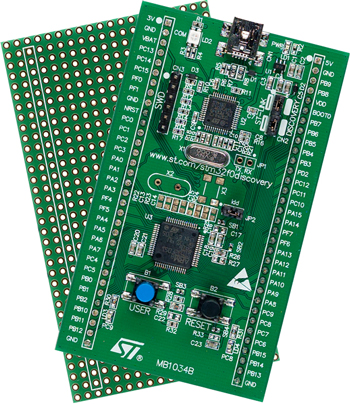
\includegraphics[scale=0.56]{stm32f0discovery}
		\end{center}
		\caption{Zestaw uruchomieniowy STM32F0-Discovery}
		\label{fig:discovery_eval_board}
	\end{figure}

	\clearpage
	Na zestaw uruchomieniowy STM32F0-Discovery składają się:
	\begin{itemize}
		\item mikrokontroler stm32f051r8 z~procesorem ARM - Cortex M0,
		\item wbudowany programator-debugger\footnote{Debugger - Program komputerowy lub urządzenie służące do dynamicznej analizy programu, w~celu odnalezienia i~identyfikacji zawartych w~nich błędów, zwanych z~angielskiego bugami (robakami). Najważniejszymi funkcjami debuggera jest praca krokowa oraz możliwość odczytania wartości zmiennych w~uruchomionych programie} ST-Link V2,
		\item cztery diody LED - dwie z~nich przeznaczone są do programowania i~podłączone są do portów GPIO, pozostałe dwie oznaczają podłączone napięcie zasilania oraz stan komunikacji USB,
		\item dwa przyciski - jeden programowalny a drugi służący do resetowania układu.
	\end{itemize}

		\section{Odbiór i~interpretacja wiadomości protokołu DDE}
		Pierwszym zadaniem sterownika będzie odebranie i~rozkodowanie ramki danych protokołu DDE poprzez port szeregowy i~sprawdzenie poprawności odebranych współrzędnych. 

			\subsection{Konfiguracja modułu transmisji szeregowej}
			Po pierwsze należy skonfigurować sam port szeregowy do pracy z~określonymi parametrami i~generującym odpowiednie przerwania.

				\paragraph{RCC - Szyny zegarowe}
				\label{sec:usart_rcc}
				Pierwszym krokiem konfiguracji modułu transmisji szeregowej było dołączenie modułu USART1 do odpowiadającej mu szyny zegarowej APB2. Podobnie szyna zegarowa AHB powinna zostać dołączona do portu GPIOA na którym znajdują się piny połączone z~modułem USART1.

				\paragraph{GPIO - Piny I/O}
				Następnie należy skonfigurować odpowiednie piny I/O, które odpowiadają modułowi USART1. Są to piny 9 i~10 portu A. Ustawione zostały w~tryb alternatywnego działania. Ich podstawową funkcją jest zwykły port wejścia/wyjścia. Jednak z~jednego pinu w~zależności od konfiguracji korzysta jeden z~kilku modułów. I~tak na przykład podstawową funkcją pinu PA9 jest I/O, a jego alternatywnymi funkcjami są:
				\begin{enumerate}
					\item nadajnik modułu USART1,
					\item drugi kanał timera TIM1,
					\item break input (wejście hamujące) timera TIM15,
					\item jedno z~wejść modułu wykrywania dotyku.
				\end{enumerate}
				W~takim przypadku należy użyć funkcji konfigurującej funkcje alternatywne dla pinów 9 i~10 - w~obydwu przypadkach na \texttt{GPIO\_AF\_1}, czyli pierwszy z~trybów pracy alternatywnej wybranych pinów (nadajnik i~odbiornik modułu USART1).

				Pozostało jeszcze skonfigurować sam port, aby oznaczył te piny jako pracujące w~trybie alternatywnym, pracujące z~częstotliwością 50MHz oraz to, aby miały wewnętrzne podciągnięcie do wysokiego stanu logicznego. Wszystko to konfigurowane jest poprzez przypisanie odpowiednich wartości do struktury inicjalizacyjnej GPIO a następnie przekazanie jej do funkcji inicjalizującej odpowiedni port. 

				\paragraph{USART - Moduł komunikacyjny}
				Kolejnym krokiem było skonfigurowanie samego modułu USART1. Do struktury inicjalizacyjnej USART zostały wpisane taka sama prędkość transmisji szeregowej (9600 bodów), a także:
				\begin{itemize}
					\item Długość słowa - 8 bitów
					\item Bity stopu - 1
					\item Bit parzystości - NIE
					\item Sprzętowa kontrola przepływu - NIE
					\item Tryby pracy - Rx (Odbiornik) i~Tx (Nadajnik)
				\end{itemize}
				Po przekazaniu tej struktury do funkcji inicjalizującej ostatnią czynnością jest wydanie polecenia włączenia modułu.

				\paragraph{NVIC - Sterownik przerwań}
				Ostatnim etapem konfiguracji transmisji szeregowej to skonfigurowanie sterownika przerwań aby reagował na przerwanie o~zapełnionym rejestrze odbiorczym wygenerowane z~modułu USART1.

			\subsection{Protokół DDE}
			Protokół DDE w~przypadku sterowania rotorem antenowym jest bardzo prosty. Przesyłany jest jeden rodzaj danych w~ustalonym formacie. Komunikat zaczyna się od litery 'W', po której wysyłane są obliczone współrzędne horyzontalne - kolejno azymut i~elewacja oddzielone pojedynczą spacją - w~formacie 3 cyfrowym z~początkowymi zerami. To znaczy, że nieważne jakiego rzędu będzie przykładowo liczba mówiąca o~współrzędnej azymutu, zawsze zostanie zapisana w~formacie trzycyfrowym. Dla przykładu: Współrzędna 235$^{\circ}$ zostanie zapisana jako 235, a współrzędna 35$^{\circ}$ jako 035. Komunikat DDE kończy się znakiem ,,powrotu karetki''\footnote{CR (Carriage Return) - znak powrotu karetki, czyli przesunięcia kursora w~terminalu bądź głowicy drukarki do początku linijki. W~językach programowania jest zazwyczaj oznaczany jako ,,\textbackslash r''}.

			\subsection{Procedura obsługi przerwania}
			\label{ssec:usart_irq_handle}
			Zadaniem procedury obsługi przerwania od modułu transmisji szeregowej jest prawidłowe odczytanie kolejnych znaków komunikatu DDE, zapisanie ich do odpowiedniego bufora tymczasowego, a ostatecznie po odebraniu znaku końca paczki danych rozkodowanie współrzędnych z~przesłanego komunikatu, sprawdzenie ich poprawności i~zapisanie do właściwych zmiennych. 

			Przerwanie od USART zostało zrealizowane jako maszyna 3 stanów.
			\begin{enumerate}
				\item Oczekiwanie na znak 'W' - początku komunikatu DDE
				\item Stan wczytywania - pobierania kolejnych znaków komunikatu DDE
				\item Wykryty błąd
			\end{enumerate}
			Sterownik ustawiany jest w~stan wczytywania tylko po odczytaniu znaku początku komunikatu DDE. Stan oczekiwania ustawiany jest zaraz po uruchomieniu sterownika, po odczytaniu symbolu końca komunikatu DDE oraz po wykryciu błędu. Stan wykrycia błędu ustawiany jest i~sprawdzany w~celu zabezpieczenia przed ustawieniem losowych sygnałów na wejścia serwomechanizmów. Błąd wykrywany jest, gdy któryś ze znaków komunikatu danych ma nieodpowiedni typ (np. w~miejscu cyfry stoi litera), gdy paczka danych przekroczy swoją domyślną długość przed otrzymaniem znaku końca komunikatu oraz gdy odczytane współrzędne nie należą do odpowiedniego zakresu.

			Po otrzymaniu znaku końca paczki danych, komunikat zostaje rozkodowany za pomocą dwóch funkcji \texttt{parse\_azimuth()} i~\texttt{parse\_altitude()}. Funkcja \texttt{parse\_azimuth()} przedstawiona została poniżej, funkcja \texttt{parse\_elevation()} wygląda analogicznie z~jednym wyjątkiem - odwołuje się do innych elementów tablicy-bufora.

			\lstinputlisting[language=C, firstline=99, lastline=115, frame=single, caption=Kod funkcji parse\_azimuth()]{interrupts.c}

			Przed zapisem dane są sprawdzane funkcją \texttt{is\_coordinates\_correct()}.
			\lstinputlisting[language=C, firstline=135, lastline=143, frame=single, caption=Kod funkcji is\_coordinates\_correct()]{interrupts.c}

			Funkcje wywołane w~\texttt{is\_coordinates\_correct()} sprawdzają czy odebrany azymut jest z~zakresu 0$^{\circ}$ - 360$^{\circ}$, oraz czy odebrana elewacja jest z~zakresu 0$^{\circ}$ - 90$^{\circ}$.

			Tak odczytane zmienne są odpowiednio zapisane i~będą użyte do ustawienia pozycji serwomechanizmów. Ta kwestia zostanie ponownie poruszona w~części~\ref{sec:servo_steering}, gdzie zostanie opisane sterowanie serwomechanizmami. 

		\section{Przyciski sterujące}
		Wprowadzenie do systemu przycisków było konieczne. Serwomechanizmy mają ograniczony zakres obrotu więc mogą być skierowane tylko w~określonym kierunku, a także potrzebna jest początkowa kalibracja anteny, aby powiadomić sterownik, gdzie antena ,,patrzy''.

			\subsection{Logika działania przycisków}
			Do sterownika podłączone zostały dwa przyciski. Jeden z~nich po kliknięciu wprowadza sterownik w~tryb opcji i~pozwala na wybranie jednego z~4 stron świata, w~którą zwrócona będzie antena. Każde kolejne naciśnięcie przycisku wybiera kolejną opcję trzymając się kolejności Północ-Wschód-Południe-Zachód. Serwomechanizm ustawiony jest w~tym trybie na środek swojego zakresu, dzięki czemu można skalibrować pozycję anteny. Drugi przycisk akceptuje aktualnie wybraną konfigurację i~wprowadza sterownik w~tryb normalnej pracy.

			\subsection{Konfiguracja portów do obsługi przycisków}
			Aby wydawanie sterownikowi poleceń było możliwe za pomocą przycisków, należy przeprowadzić odpowiednią konfigurację na co składa się włączenie odpowiednich zegarów, konfiguracja portu I/O, dołączenie modułu przerwań zewnętrznych EXTI\footnote{EXTI (EXTernal Interrupts - Przerwania zewnętrze, to znaczy nie wygenerowane przez żadnej z~modułów wewnętrznych mikrokontrolera, lecz wygenerowane na podstawie zdarzeń zaistniałych na pinach GPIO)} oraz włączenie opcji obsługi przerwań w~module NVIC.

				\paragraph{RCC - Szyny zegarowe}
				Przyciski zostały dołączone do portu GPIOB, więc port ten powinien zostać przyłączony do szyny zegarowej AHB. W~celu zastosowania sterownika przerwań zewnętrznych należy także dołączyć do szyny zegarowej APB2 moduł SYSCFG, który (pomimo mylącej nazwy) odpowiada za taktowanie sterownika przerwań zewnętrznych.

				\paragraph{GPIO - Piny I/O}
				Drugim krokiem jest konfiguracja samych pinów I/O do pracy jako wejścia. W~tym celu należy uzupełnić strukturę inicjalizacyjną GPIO żądanymi parametrami. W~projekcie przyciski podłączone są do pinów 2 i~3 portu GPIOB. Tryb pracy tych pinów został ustawiony jako wejściowy z~częstotliwością pracy 50MHz. Same piny zostały wewnętrznie podciągnięte do wysokiego stanu napięciowego. Ta struktura została przekazana następnie do funkcji inicjalizacyjnej.

				\paragraph{EXTI}
				Kolejnym etapem było skonfigurowanie sterownika przerwań zewnętrznych EXTI. Sterownik ten konfiguruje linie przerwań w~zależności od numeru pinu a niezależnie od portu do jakiego pin ten należy. To znaczy, że to samo przerwanie wygeneruje pin 2 portu A, co pin 2 portu B. Należy więc odpowiednio ustawić dwie linie przerwań EXTI - linię 2 i~linię 3. Przerwanie będzie wyzwalane rosnącym zboczem, co skutkuje tym, że procedura obsługi przerwania wykonywana będzie w~momencie puszczania klawisza sterującego.

				Ostatecznie należy poinformować sterownik EXTI, aby reagował na zmiany napięć na odpowiednich pinach poleceniami:

				\begin{lstlisting}[language=C, frame=single, caption=Dowiązanie pinów do sterownika EXTI]
SYSCFG_EXTILineConfig(EXTI_PortSourceGPIOB, EXTI_PinSource2);
SYSCFG_EXTILineConfig(EXTI_PortSourceGPIOB, EXTI_PinSource3);
				\end{lstlisting}

				\paragraph{NVIC - Sterownik przerwań}
				Ostatnim etapem było dodanie konfiguracji EXTI do sterownika przerwań NVIC. W~sterowniku EXTI linię 2 i~3 obsługuje jeden kanał przerwań nazwany \texttt{EXTI2\_3\_IRQn}. To znaczy, że należy zaimplementować tylko jedną procedurę obsługi przerwania EXTI - \texttt{EXTI2\_3\_IRQHandler}, a następnie już w~samej procedurze rozróżniać, która linia to przerwanie wywołała.

				Kanał przerwań \texttt{EXTI2\_3\_IRQn} zdefiniowany został w~sterowniku NVIC z~priorytetem niższym od przerwania od modułu USART. Szybkie odebranie i~przetworzenie danych jest ważniejsze od ustawienia trybu pracy sterownika.


			\subsection{Konfiguracja portów do obsługi diod LED}
			W~sytuacji, gdy sterownik umożliwia sterowanie jego trybami oraz opcjami, musi zwracać informację użytkownikowi o~swoim obecnym stanie. W~tym celu zostały wykorzystane diody LED. Dwie z~nich oznaczają tryb pracy sterownika - tryb normalnej pracy (kolor zielony) i~tryb kalibracji (kolor żółty) oraz kolejne cztery oznaczające wybraną stronę świata, w~którą skierowana jest antena (kolor niebieski).

				\paragraph{RCC - Szyny zegarowe}
				Diody zostały podłączone do portu GPIOA, który został już wcześniej podłączony do właściwej szyny zegarowej w~podpunkcie~\ref{sec:usart_rcc}.

				\paragraph{GPIO - Piny I/O}
				Piny 0-5 portu GPIOA zostały włączone a ich tryb pracy został ustawiony na wyjściowy z~częstotliwością pracy 50MHz.

			\subsection{Procedura obsługi przerwania zewnętrznego}
				Po wystąpieniu przerwania spowodowanego wciśnięciem odpowiedniego przycisku pierwszą czynnością jest rozróżnienie, który przycisk je wywołał. W~przypadku przycisku podłączonego do pinu 2 (akceptowanie opcji), zmieniany jest wyłącznie stan sterownika na tryb normalnej pracy. To pozwala innym funkcjom i~procedurom na normalne ustawianie pozycji serwomechanizmów. Przycisk podłączony do pinu 3 (zmiana kierunku anteny) wywołuje funkcję, która zmienia stan sterownika na tryb kalibracji i~wpisuje do zmiennej kolejny z~dostępnych kierunków ustawienia anteny.

				Po zmianie wartości zmiennych odpowiadających za stan sterownika i~kierunek ustawienia anteny wywoływana jest funkcja, która włącza lub wyłącza diody zgodnie z~ich przeznaczeniem.

				Po zakończeniu procedury, resetowana jest flaga obsługiwanego przerwania. W~przeciwnym razie sterownik zapętliłby się na jego obsłudze uniemożliwiając normalną pracę a co za tym idzie brak reakcji ze strony sterownika na nowe komunikaty sterujące. Jest to jeden z częstszych błędów w przypadku programowania aplikacji używających przerwań zewnętrznych i jednocześnie jednym z trudniejszych do zlokalizowania bez inspekcji rejestrów mikrokontrolera w czasie działania programu.

		\section{Sterowanie serwomechanizmem}
		\label{sec:servo_steering}
			\begin{wrapfigure}{r}{0.4\textwidth}
				\vspace{-20pt}
				\begin{center}
					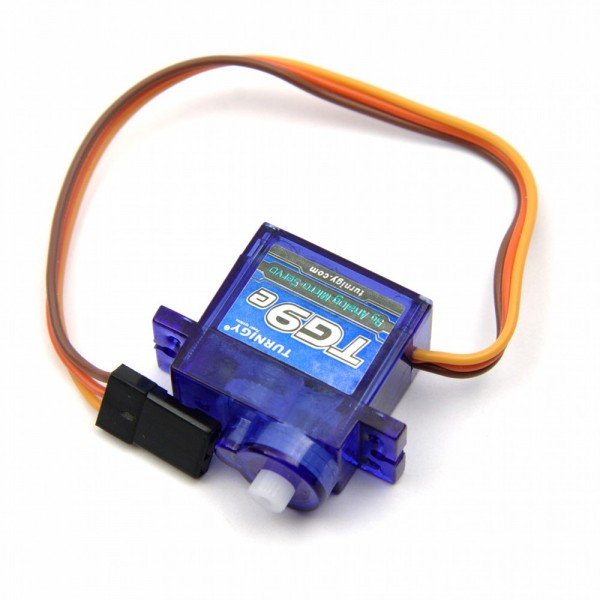
\includegraphics[width=0.4\textwidth]{servo}
				\end{center}
				\vspace{-20pt}
				\caption{Serwomechanizm Turnigy TG9e użyty w~projekcie}
				\vspace{-10pt}
				\label{fig:servo}
			\end{wrapfigure}
		Aby sterować anteną, należy ustawić w~odpowiedniej pozycji serwomechanizmy. Po pierwsze nietypowa jest sama zasada sterowania serwomechanizmami. Ważnym jest także zbadanie parametrów serwomechanizmów dostępnych do stworzenia projektu. Do zbudowania gotowego urządzenia wykorzystane zostały tanie serwomechanizmy modelarskie - Turnigy TG9e. Mają one małą moc, jednak są w~stanie obracać lekką antenę typu Arrow i~będą wystarczające do zastosowania ich w~terenie do łączności satelitarnych. Kolejną czynnością będzie ustawienie modułu sterownika STM32F0-Discovery, który odpowiedzialny jest za generowanie wymaganego przez serwomechanizmy sygnału. Następnym krokiem sterowania jest obliczenie parametrów sygnału do odpowiedniego ustawienia anteny. Ostatnim zadaniem będzie powiązanie danych z~odczytanego komunikatu DDE z~funkcjami zmieniającymi parametry sygnału sterującego serwomechanizmami.

			\subsection{Co to jest serwomechanizm}
			Serwomechanizm jest to zamknięty układ sterowania ze sprzężeniem zwrotnym składający się z~prostego silnika prądu stałego z~dodatkowymi przekładniami oraz układem sterującym. Układ sterujący składa się z~potencjometru sprzężonego z~wałem, do którego przymocowane jest ramię serwomechanizmu, oraz układem regulacji. Układ sterujący może dokładnie stwierdzić w~jakiej pozycji znajduje się wał. Dzięki temu można z~dużą dokładnością prozycjonować wał. W~większości przypadków wał serwomechanizmu może przyjmować pozycje kątowe z~zakresu 0-180$^{\circ}$. Większość serwomechanizmów posiada ograniczniki, które nie pozwalają na większe wychylenia wału. Ze światem zewnętrznym serwomechanizm jest połączony za pomocą trzech przewodów - zasilania (czerwony), potencjału zerowego (czarny) oraz sygnał sterujący (biały lub żółty).

			\subsection{Zasada sterowania serwomechanizmem modelarskim}
			Serwomechanizmy sterowane są poprzez jedną linię sygnałową, na którą należy podać sygnał PWM o~ustalonych parametrach. Układ sterujący wbudowany w~serwomechanizm posiada generator ustawiony na 50Hz, czyli co 20ms należy podać na linię sterującą sygnał o~odpowiedniej długości. Większość serwomechanizmów ustawia wał w~pozycji centralnej dla impulsu o~długości 1,5ms. Końce zakresy osiągają dla impulsów od 1ms do 2ms. Jednak różni producenci określają różne zakresy sygnału, co powinni określić w~nocie katalogowej urządzenia. Niestety po długich poszukiwaniach noty katalogowej dla serwomechanizmu wykorzystanego w~projekcie, znalezione zostały tylko sprzeczne informacje na prywatnych stronach internetowych hobbystów. W~związku z~tym zbadano parametry serwomechanizmu ręcznie, co zostało opisane w~podpunkcie~\ref{ssec:servo_analysis}. Linie zasilania należy dołączyć do osobnego źródła o~napięciu 5V. Nie mogą być one podłączone do sterownika, gdyż działa on w~zakresie napięć 0V - 3.3V, co generuje za mało mocy aby poruszać serwomechanizmem.

			\subsection{Konfiguracja modułu generującego sygnał PWM}
			Sygnał PWM jest generowany z~modułu timera TIM1 ustawionego w~tryb generowania sygnału PWM. Wyjścia jego 4 kanałów znajdują się na pinach 8-11 portu GPIOA. Ze względu na to, że piny 9 i~10 zostały już wykorzystane na komunikację szeregową USART, jako wyjścia z~wygenerowanym sygnałem PWM zostały wykorzystane piny 8 i~11 czyli pierwszy i~czwarty kanał timera TIM1. 

				\paragraph{RCC - Szyny zegarowe}
				Serwomechanizmy zostały podłączone do portu GPIOA, który został już wcześniej podłączony do właściwej szyny zegarowej w~podpunkcie~\ref{sec:usart_rcc}. Dodatkowo do szyny zegarowej APB2 został podłączony moduł timera TIM1.

				\paragraph{GPIO - Piny I/O}
				Pierwszym krokiem konfiguracji GPIO było włączenie pinów 8 i~11 do pracy w~trybie funkcji alternatywnych z~częstotliwością 50MHz. Następnie funkcje alternatywne tych pinów zostały ustawione na obsługę modułu timera TIM1. W~tym wypadku na drugi tryb funkcji alternatywnych \texttt{GPIO\_AF\_2}.

				\paragraph{TIM - Moduł timera}
				Ostatecznie pozostało skonfigurować sam moduł timera. Po pierwsze został ustawiona część odpowiadająca za podstawę czasu. Ponieważ domyślnie mikrokontroler stm32f051r8 jest taktowany zegarem o~częstotliwości 48MHz, a rejestr timera jest 16-bitowy (jego rejestr może przyjąć 65536 wartości). Skutkiem tego okresy sygnału PWM byłyby za krótkie. W~tym wypadku należało użyć preskalera wbudowanego w~moduł timera. Daje to możliwość naliczania przez timer odpowiednio wielokrotności taktów zegara procesora. Preskaler ustawiony został, aby naliczać do 48 takt zegara procesora, czyli co jedną mikrosekundę. Serwomechanizm wymaga sygnału z~okresem 20 milisekund, więc rejestr przepełnienia timera został ustawiony na 20000. W~ten sposób co 20ms rozpoczyna nowy cykl sygnału PWM.

				Po ustawieniu podstawy czasu timera TIM1, przyszedł czas na samą konfigurację jego pracy. Jego tryb został ustawiony na generowanie sygnału PWM z~nieaktywnym stanem niskim oraz aktywnym stanem wysokim. W~przypadku odwrotnej konfiguracji stanów aktywnych i~nieaktywnych generowany sygnał byłby zanegowany w~stosunku do żądanego. Ostatnim parametrem jest długość pulsu sygnału. Początkowo ustawiony został na domyślny środkowy punkt serwomechanizmu, czyli 1500 - co daje puls długości 1,5ms.

				Takimi parametrami zostały zainicjalizowane obydwa używane kanały timera TIM1. Układy timera powinny zostać jeszcze włączone, a także włączony powinien zostać moduł generacji sygnału PWM. Bez tych dwóch komend na wyjściach mikrokontrolera nie pojawi się żaden sygnał.

			\subsection{Badanie dostępnych serwomechanizmów}
			\label{ssec:servo_analysis}
			Serwomechanizmy musiały zostać przebadane pod względem zależności ustawienia kąta wychylenia ramienia od długości impulsu sygnału wejściowego. Na potrzeby tego badania został skonstruowany osobny układ, który odbierał przez port szeregowy wartości dla długości pulsu a następnie generował dany sygnał PWM na wejście sterujące serwomechanizmu. Przeprowadzane badania pozwoliły ustalić długości impulsu PWM dla pozycji środkowej serwomechanizmu oraz kątów wychylenia 45$^{\circ}$ i~90$^{\circ}$ w~obie strony. To pozwoliło zaobserwować charakterystykę serwomechanizmów - która okazała się być bardzo zbliżona do liniowej.

			\paragraph{Wyniki badań [Wychylenie ramienia - szerokość impulsu]}
			\begin{description}
			\item[-90$^{\circ}$] - 2,70 ms
			\item[-45$^{\circ}$] - 2,10 ms
			\item[0$^{\circ}$] - 1,55 ms
			\item[45$^{\circ}$] - 1,00 ms
			\item[90$^{\circ}$] - 0,60 ms
			\end{description}

			\subsection{Obliczenia i sterowanie}
			Początkowym obliczeniem jest wyliczenie odebranego od programu Orbitron azymutu z~poprawką na ustawienie anteny pod względem strony świata, czyli kątu względem ustawienia centralnego serwomechanizmu. Kąt ten obliczany jest odejmując azymut początkowego ustawienia anteny od azymutu odebranego przez sterownik.
			
			Funkcja ustawiająca pozycję serwomechanizmu pobiera w~argumencie wychylenie względem pozycji środkowej. Potrzebne jest więc proste przekształcenie. Współrzędne większe niż 180$^{\circ}$ należy pomniejszyć o~360. W~ten sposób otrzymuje się pożądane wychylenie względem pozycji środkowej serwomechanizmu.

			Dalszymi operacjami zajmują się już funkcje obsługi serwomechanizmu. Dla podanego kąta wychylenia obliczane są szerokości impulsów PWM dla obydwu serwomechanizmów, a następnie te wartości przekazywane są do kolejnej funkcji, która aktualizuje rejestry kanałów 1 i~4 timera TIM1.

			\subsection{Automatyzacja sterowania serwomechanizmami}
			Ostatnim krokiem jest dołączenie do procedury obsługi przerwania, opracowanej w~podpunkcie~\ref{ssec:usart_irq_handle}, wywołania funkcji ustawiającej ramie serwomechanizmu w~żądanej pozycji. Wywołanie tej funkcji zostało umieszczone we fragmencie kodu, który wykonuje się gdy odebrany zostanie koniec komunikatu DDE, współrzędne zostaną sparsowane i~zostanie sprawdzona ich poprawność.

	\chapter{Obsługa urządzenia}
	\label{sec:how_to_use_device}
	Samo urządzenie działa od momentu podłączenia go do zasilania. Początkowo jest ustawiane w~tryb kalibracji i~domyślnie ustawionym kierunkiem anteny na północ. W~tym momencie możliwa jest zmiana kierunku anteny oraz potwierdzenie swojego wyboru, co skutkuje przejściem sterownika do trybu normalnej pracy. Serwomechanizmy ustawią się w~poprawnej pozycji w~momencie otrzymania pierwszego właściwego komunikatu protokołu DDE od programu Orbitron. Ostatnim krokiem jest uruchomienie i~konfiguracja programu Orbitron w~parze ze sterownikiem WispDDE, a następnie wybranie żądanej anteny, która aktualnie przelatuje lub będzie przelatywać w~zasięgu anteny.

		\section{Przygotowanie oprogramowania komputerowego}
		
			\subsection{Konfiguracja programu Orbitron}
			Koniecznymi ustawieniami w~programie Orbitron są:
			\begin{enumerate}
				\item współrzędne geograficzne położenia anteny,
				\item wysokość nad poziomem morza (konieczna do korekcji elewacji),
				\item wybór sterownika DDE.
			\end{enumerate}

			Współrzędne geograficzne oraz wysokość ustawia się w~zakładce Lokalizacja. Długość i~szerokość geograficzną można wpisać ręcznie w~pola tekstowe lub wybrać z~już zdefiniowanych profili. Wysokość nad poziomem morza należy wpisać ręcznie w~pole tekstowe. Po ustawieniu koniecznych opcji lokalizacji, konfigurację można zapisać na liście konfiguracji prywatnych.

			\subsection{Wybór sterownika DDE}				
			\begin{figure}[!htb]
				\begin{center}
					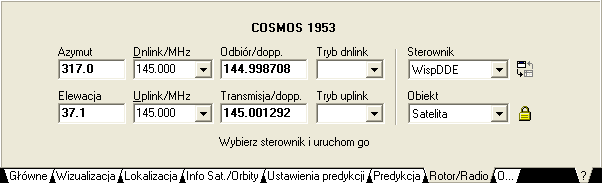
\includegraphics[scale=0.7]{screen2}
				\end{center}
				\caption{Orbitron - Ustawienia sterownika DDE}
				\label{fig:DDE_settings}
			\end{figure}
			Do komunikacji programu Orbitron ze światem zewnętrznym, a w~szczególności ze sterownikiem antenowym - koniecznym jest użycie zewnętrznego sterownika do transmisji danych (DDE). W~tym wypadku użyty został sterownik WispDDE. Należy go wybrać z~listy sterowników w~zakładce Rotor/Radio programu Orbitron tak jak to jest widoczne na rysunku~\ref{fig:DDE_settings}. Po dokonaniu wyboru, należy kliknąć przycisk znajdujący się obok listy uruchamiający sterownik. Może się zdarzyć, że program Orbitron nie będzie mógł zlokalizować sterownika na komputerze i~poprosi o~ręczne wskazanie jego położenia na dysku.
		
			\begin{figure}[!htb]
				\centering
				\begin{subfigure}[b]{0.4\textwidth}
					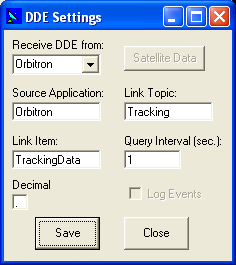
\includegraphics[scale=0.7]{screen4}
					\caption{WispDDE - DDE Link}
					\label{fig:WispDDE_DDE_Link_settings}
				\end{subfigure}
				\begin{subfigure}[b]{0.4\textwidth}
					\begin{center}
						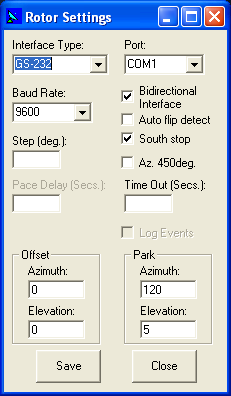
\includegraphics[scale=0.7]{screen5}
						\caption{WispDDE - Rotor}
						\label{fig:WispDDE_Rotor_settings}
					\end{center}
				\end{subfigure}
				\caption{WispDDE - Okna konfiguracji sterownika WispDDE}
			\end{figure}

			Po uruchomieniu sterownika przez program Orbitron, należy przeprowadzić jego krótką, wstępną konfigurację. Po pojawieniu się głównego okna programu należy sprawdzić, czy sterownik poprawnie odebrał dane od programu Orbitron i~wyświetlił nazwę wybranej satelity. Następnie z~menu \texttt{Settings} wybieramy okno \texttt{DDE Link} przestawione na rysunku~\ref{fig:WispDDE_DDE_Link_settings} i~wybieramy takie same opcje. 
			Po zapisaniu tych ustawień, przechodzimy do kolejnego okna ustawień sterownika DDE wybierając z~menu \texttt{Settings} pozycję \texttt{Rotor}. W~tym oknie należy wybrać opcję interfejsu komunikacyjnego, portu oraz szybkości transmisji jak na rysunku~\ref{fig:WispDDE_Rotor_settings}. Konfiguracja użyta w~projekcie to:
			\begin{itemize}
				\item Interface Type - GS-232
				\item Port - COM1
				\item Baud Rate - 9600
			\end{itemize}

			Na tym etapie na wybrany port szeregowy wysyłane będą ramki protokołu DDE z~obliczonymi współrzędnymi horyzontalnymi do ustawienia anteny.

	\chapter{Podsumowanie}
	\label{sec:summit}
	W~projekcie zostały spełnione założenia, które zostały przedstawione w~rozdziale~\ref{sec:problem_description}. Sterownik automatycznie ustawia pozycję anteny w~kierunku wybranej przez użytkownika satelity. Cały system jest tani, w~połączeniu z~lekkimi antenami typu Arrow jest także bardzo mobilny (ze względu na swoją wagę i~stopień skomplikowania konstrukcji). Po ustawieniu i~skalibrowaniu sterownika, użytkownik systemu może wybrać dowolną antenę w~świetle zasięgu anteny. Wtedy system nie tylko skieruje antenę w~kierunku wybranej satelity, ale będzie ją śledził dopóki będzie miał ją w~swoim zasięgu. Tanie serwomechanizmy mają pewien margines swojej dokładności, ale zważając na to, że tolerancja anteny to około 4$^{\circ}$, jest to zupełnie akceptowalne.

	Projekt ten posiada dużo możliwości rozwoju. Jednym z najciekawszych jest dodanie akcelerometru i magnetometru. To zwiększyłoby możliwości oraz ułatwiłoby pozycjonowanie anteny. Dodatkowo ważnym elementem systemu jest komunikacja z~użytkownikiem. W~obecnej wersji projektu komunikuje się on systemem za pomocą klawiszy i~odczytuje od niego informacje za pomocą diod LED. Rozszerzeniem tego byłoby wbudowanie pokręteł (najlepiej zrealizowanych na impulsatorach obrotowych) oraz wyświetlacza alfanumerycznego lub graficznego. To zwiększyłoby przejrzystość i~czytelność interfejsu i~sprawiłoby sterowanie systemem bardziej intuicyjnym. 

	Oczywiście są także elementy systemu, które mogłyby zostać poprawione. W projekcie zostały zastosowane najtańsze serwomechanizmy ogólnie dostępne na rynku części modelarskich. To przekłada się na ich udźwig oraz dokładność. Same serwomechanizmy mogłyby też zostać wymienione na małe i~lekkie silniki krokowe. To zwiększyłoby dokładność systemu. To jednak może być zbyt drogie w~stosunku do założeń. Jak zostało już wspomniane, anteny mają pewną tolerancję, więc zbyt ,,droga'' dokładność nie jest wskazana.

	\nocite{*}
	\addcontentsline{toc}{chapter}{Bibliografia}
	\bibliography{bibliografia}
	
	\listoffigures

\end{document}
